\documentclass[11pt,a4paper]{article}

\usepackage[T1]{fontenc}
\usepackage[utf8]{inputenc}
\usepackage[english]{babel}
\usepackage{lmodern}
%\usepackage{circuitikz}
\usepackage{color}
\usepackage{wrapfig}
\usepackage{placeins}
\usepackage{subfigure}
\usepackage{tabu}
\usepackage{fullpage}
\usepackage[squaren]{SIunits}
\usepackage{graphicx}
%\usepackage[pdftex]{graphicx}
\usepackage{epstopdf}
\usepackage{epsfig}
\usepackage{hyperref}
\usepackage{tikz}
\usepackage{tikz-qtree}
\usetikzlibrary{arrows}
\usepackage{eurosym}
%\usepackage{chemist}
\usepackage{amsmath}
\usepackage{amssymb}
\usepackage{mathrsfs}
\usepackage{dsfont}% use $\mathds{1}$
\newcommand{\C}{\mathbb{C}}
\newcommand{\N}{\mathbb{N}}
\newcommand{\Z}{\mathbb{Z}}
\newcommand{\R}{\mathbb{R}}
\newcommand{\red}{\textcolor{red}}
\newcommand{\dis}{\displaystyle}
\newcommand{\dr}{\partial}
\newcommand{\txt}{\text}
\newcommand{\td}{\todo[inline]}
\newcommand{\ttt}{\texttt}
\newcommand{\itt}{\textit}

\usepackage{algorithm}
\usepackage{todonotes}
\usepackage[noend]{algpseudocode}


%\newtheorem{theoreme}			     {Théorème}	[chapter]
%\newtheorem{proposition}[theoreme]	 {Proposition}	
%\newtheorem{corollaire}	  [theoreme]	 {Corollaire}	
%\newtheorem{lemme}	      [theoreme]  {Lemme}		
%\newtheorem{definition}	         {Définition}[chapter]
%\theoremstyle{definition}
%\newtheorem{exemple}			     {Exemple}	[chapter]
%\newtheorem{contreexemple}[exemple]{Contre-exemple}
%\newtheorem{probleme}	             {Probl\`eme}[chapter]

\usepackage{listings}
\usepackage{textcomp}
\definecolor{listinggray}{gray}{0.9}
\definecolor{lbcolor}{rgb}{0.9,0.9,0.9}
\lstset{
	backgroundcolor=\color{lbcolor},
	tabsize=4,
	rulecolor=,
	language=matlab,
        basicstyle=\scriptsize,
        upquote=true,
        aboveskip={1.5\baselineskip},
        columns=fixed,
        showstringspaces=false,
        extendedchars=true,
        breaklines=true,
        prebreak = \raisebox{0ex}[0ex][0ex]{\ensuremath{\hookleftarrow}},
        frame=single,
        showtabs=false,
        showspaces=false,
        showstringspaces=false,
        identifierstyle=\ttfamily,
        keywordstyle=\color[rgb]{0,0,1},
        commentstyle=\color[rgb]{0.133,0.545,0.133},
        stringstyle=\color[rgb]{0.627,0.126,0.941},
}

\DeclareMathOperator{\e}{e}

\begin{document}
\tabulinesep=1.2mm
\title{Project Assignment 1A}
\author{\today\\ SF2812 Applied Linear Optimization}
\date{
	\begin{tabular}{r c l}
		Petter Aronsson & \href{mailto:petterar@kth.se}{petterar@kth.se} & 19900910-0414\\
		Henrik Ekestam & \href{mailto:hekestam@kth.se}{hekestam@kth.se} & 19931113-5678\\
		David Weicker & \href{mailto:weicker@kth.se}{weicker@kth.se} & 940114-T115\\
	\end{tabular}
}
\maketitle


%\section*{Problem description}
The telecommunication company Nett provides capacity between cites in Europe. The cities are Stockholm, Berlin, London, Warsaw, Paris, Madrid and Rome. Some of the cities are connected in which traffic can be sent in both directions. The connections and the maximum traffic which can be sent between the cites respectively can be seen in Figure 1.

Nett wishes to provide 50 Gbit/s between Stockholm and Rome at the same time they provide 40 Gbit/s between London and Warsaw. They need help in routing the traffic because of the capacity limitations. Also, they would like to investigate if there is any slack in the network, potential to adding another traffic route and how to handle fluctuations in capacity.

\begin{center}
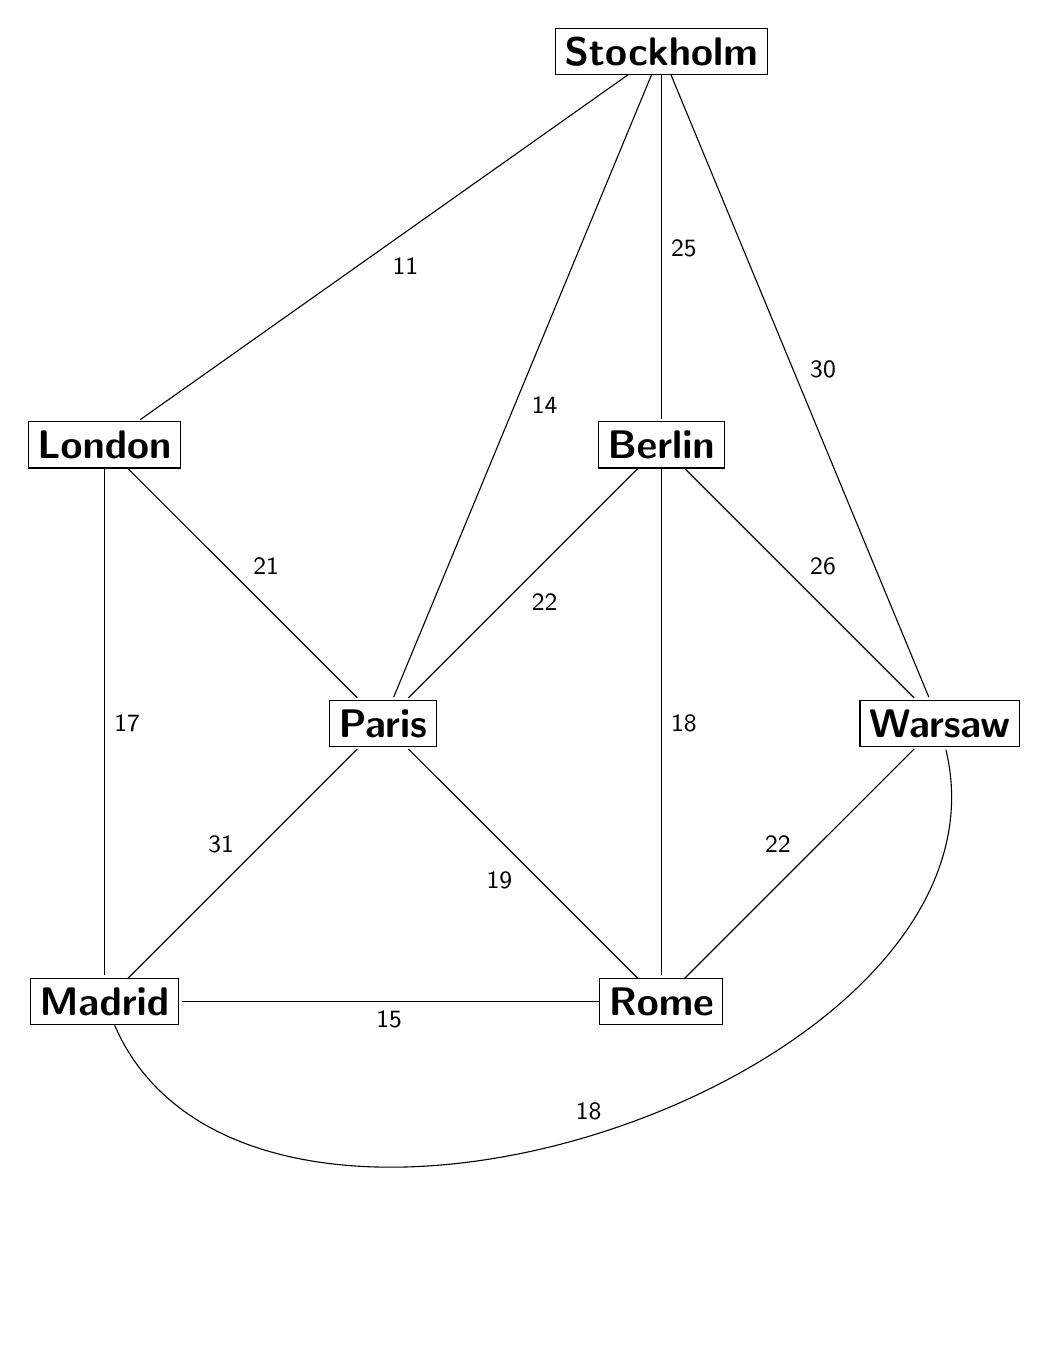
\begin{tikzpicture}[shorten >=1pt,auto,node distance=5cm,
                    main node/.style={rectangle,draw,font=\sffamily\Large\bfseries}]
  \node[main node] (1) {Stockholm};
  \node[main node] (2) [below of=1] {Berlin};
  \node[main node] (3) [below right of=2] {Warsaw};
  \node[main node] (4) [below left of=2] {Paris};
  \node[main node] (5) [above left of=4] {London};
  \node[main node] (6) [below right of=4] {Rome};
  \node[main node] (7) [below left of=4] {Madrid};

  \path[every node/.style={font=\sffamily\small}]
    (1) edge node {25} (2)
     	edge node {30} (3)
    	edge node {14} (4)
    	edge node {11} (5)
    (2) edge node {26} (3)
    	edge node {22} (4)
        edge node {18} (6)
    (5) edge node {17} (7)
        edge node {21} (4)
    (6) edge node {19} (4)
        edge node {15} (7)
        edge node {22} (3)
    (7) edge [bend right=85] node {18} (3)
    	edge node {31} (4);
  
\end{tikzpicture}
\end{center}
Figure 1. System modelled as a network where maximum capacity is marked out on the arcs.

\newpage

\section*{Routing the traffic}

\begin{center}
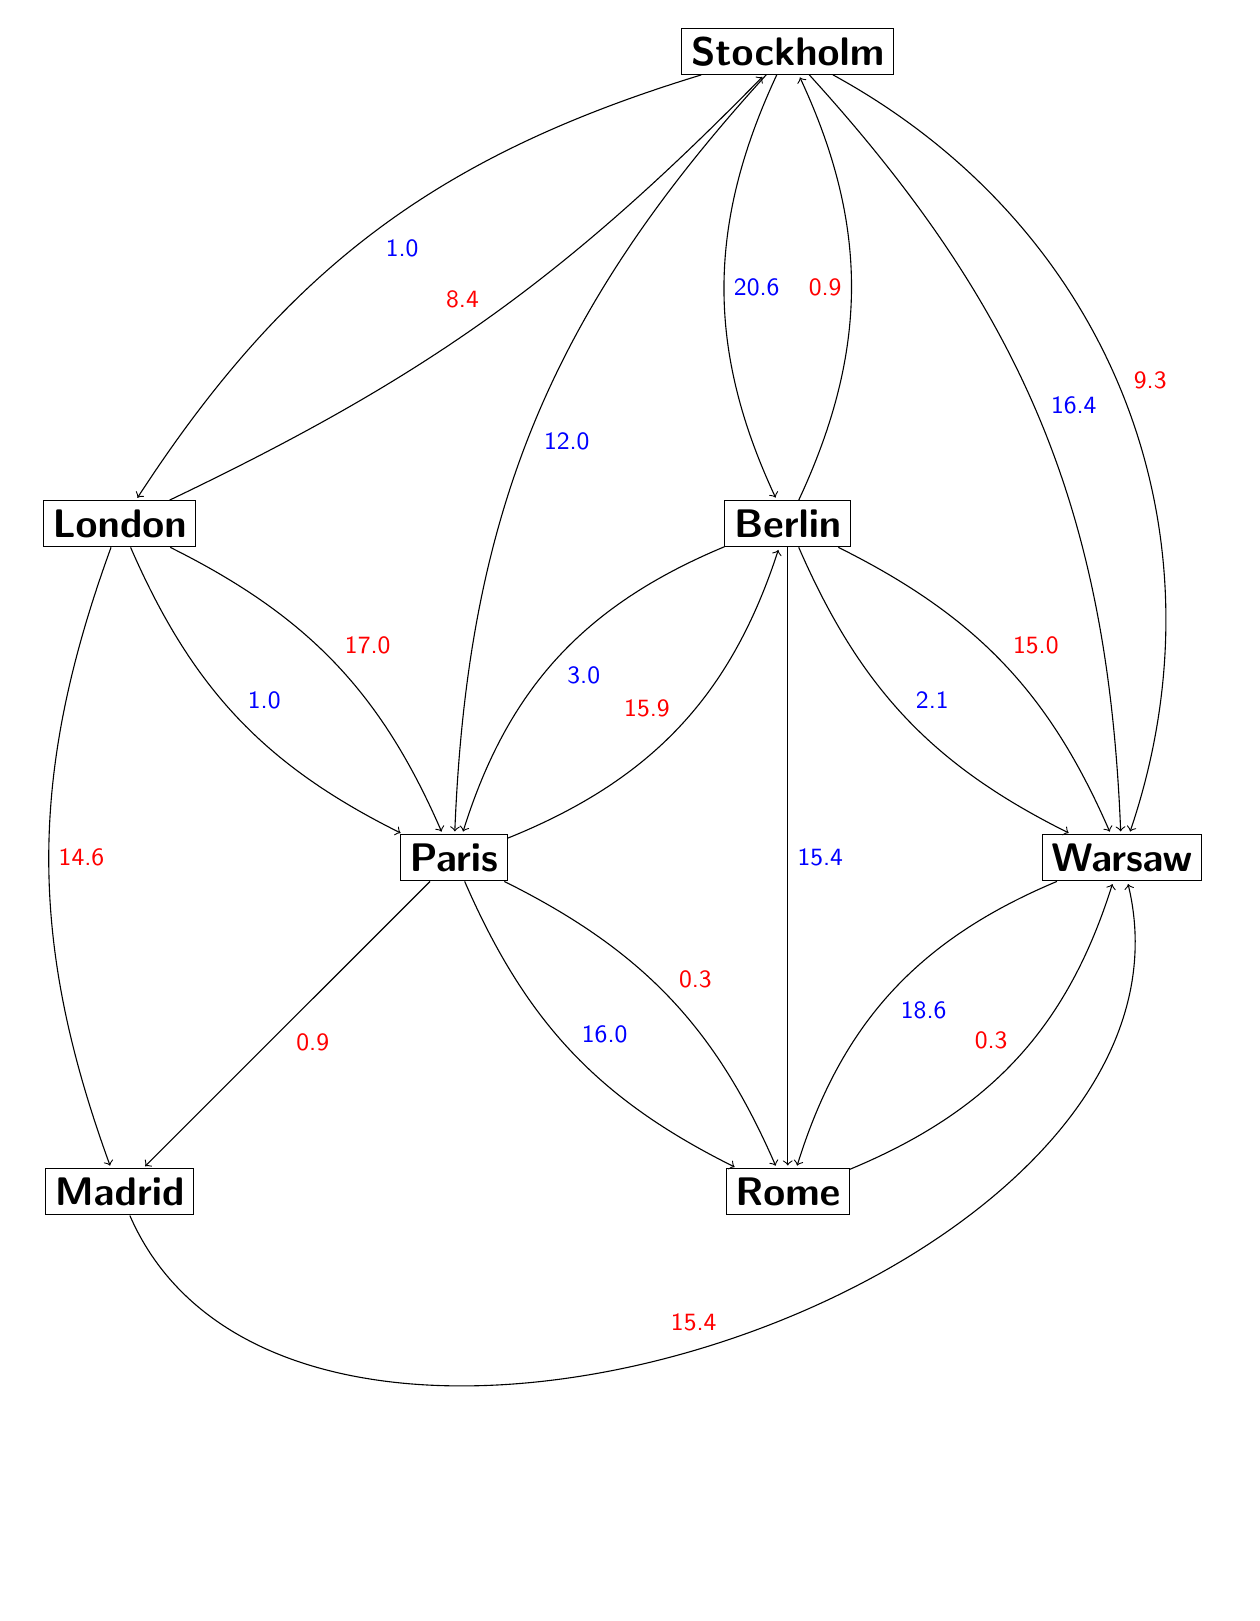
\begin{tikzpicture}[->,shorten >=1pt,auto,node distance=6cm,
                    main node/.style={rectangle,draw,font=\sffamily\Large\bfseries}]
  \node[main node] (1) {Stockholm};
  \node[main node] (2) [below of=1] {Berlin};
  \node[main node] (3) [below right of=2] {Warsaw};
  \node[main node] (4) [below left of=2] {Paris};
  \node[main node] (5) [above left of=4] {London};
  \node[main node] (6) [below right of=4] {Rome};
  \node[main node] (7) [below left of=4] {Madrid};

  \path[every node/.style={font=\sffamily\small}]
    (1) edge [bend right=20] node[blue] {1.0} (5)
    	edge [bend right=20] node[blue] {12.0} (4)
     	edge [bend right=25] node[blue] {20.6} (2)
    	edge [bend left=20] node[blue] {16.4} (3)
    	edge [bend left=40] node[red] {9.3} (3)
    (2) edge [bend right=25] node[red] {0.9} (1)
    	edge [bend right=25] node[blue] {3.0} (4)
        edge [bend right=20] node[blue] {2.1} (3)
    	edge [bend left=20] node[red] {15.0} (3)
    	edge node[blue] {15.4} (6)
    (3) edge [bend right=25] node[blue] {18.6} (6)
    (4) edge [bend right=25] node[red] {15.9} (2)
    	edge [bend right=20] node[blue] {16.0} (6)
    	edge [bend left=20] node[red] {0.3} (6)
    	edge node[red] {0.9} (7)
    (5) edge [bend right=10] node[red] {8.4} (1)
    	edge [bend left=20] node[red] {17.0} (4)
    	edge [bend right=20] node[blue] {1.0} (4)
		edge [bend right=20] node[red] {14.6} (7)
	(6) edge [bend right=25] node[red] {0.3} (3)
    (7) edge [bend right=85] node[red] {15.4} (3);
  
\end{tikzpicture}
\end{center}

\section{Model 2:}
blibli

\section{Model 3}
\subsection{Presentation of the problem}
In this section, we are going to generalize the model a little bit. Up to this point, we have considered that each link has a known capacity and that this quantity is exact. This is, however, not true in general. We can expect the actual capacities to be close to the numbers given but we should take into account that they can fluctuate around those values. Our new model will thus have to deal with this uncertainty. Because the value of the capacities can be considered as an unknown parameter, we will use stochastic programming.

We also know that the 50 Gbit/s-demand can be rerouted after the actual values are known but the 40 Gbit/s-demand must be determined on beforehand (and thus not cannot be rerouted after knowing the actual capacities).

\subsection{Mathematical model}
Just as in the previous models, we introduce the set $I$ :
$$I = \{ Sto,Lon,Ber,War,Par,Rom,Mad\}$$


 

\clearpage

\section{Results}
\subsection{Results  model 1}
This section presents the results for the different models presented above.

\subsection{Results for routing the traffic}
The solution to routing the traffic in the network when minimizing the maximum utility in any link can be seen in Figure 2. The figure shows how much of each type of traffic that is to be sent in each arc. The blue numbers, $k=1$, denotes the flow from Stockholm to Rome and the red numbers, $k=2$, denotes the flow from London to Warsaw. 

\begin{center}
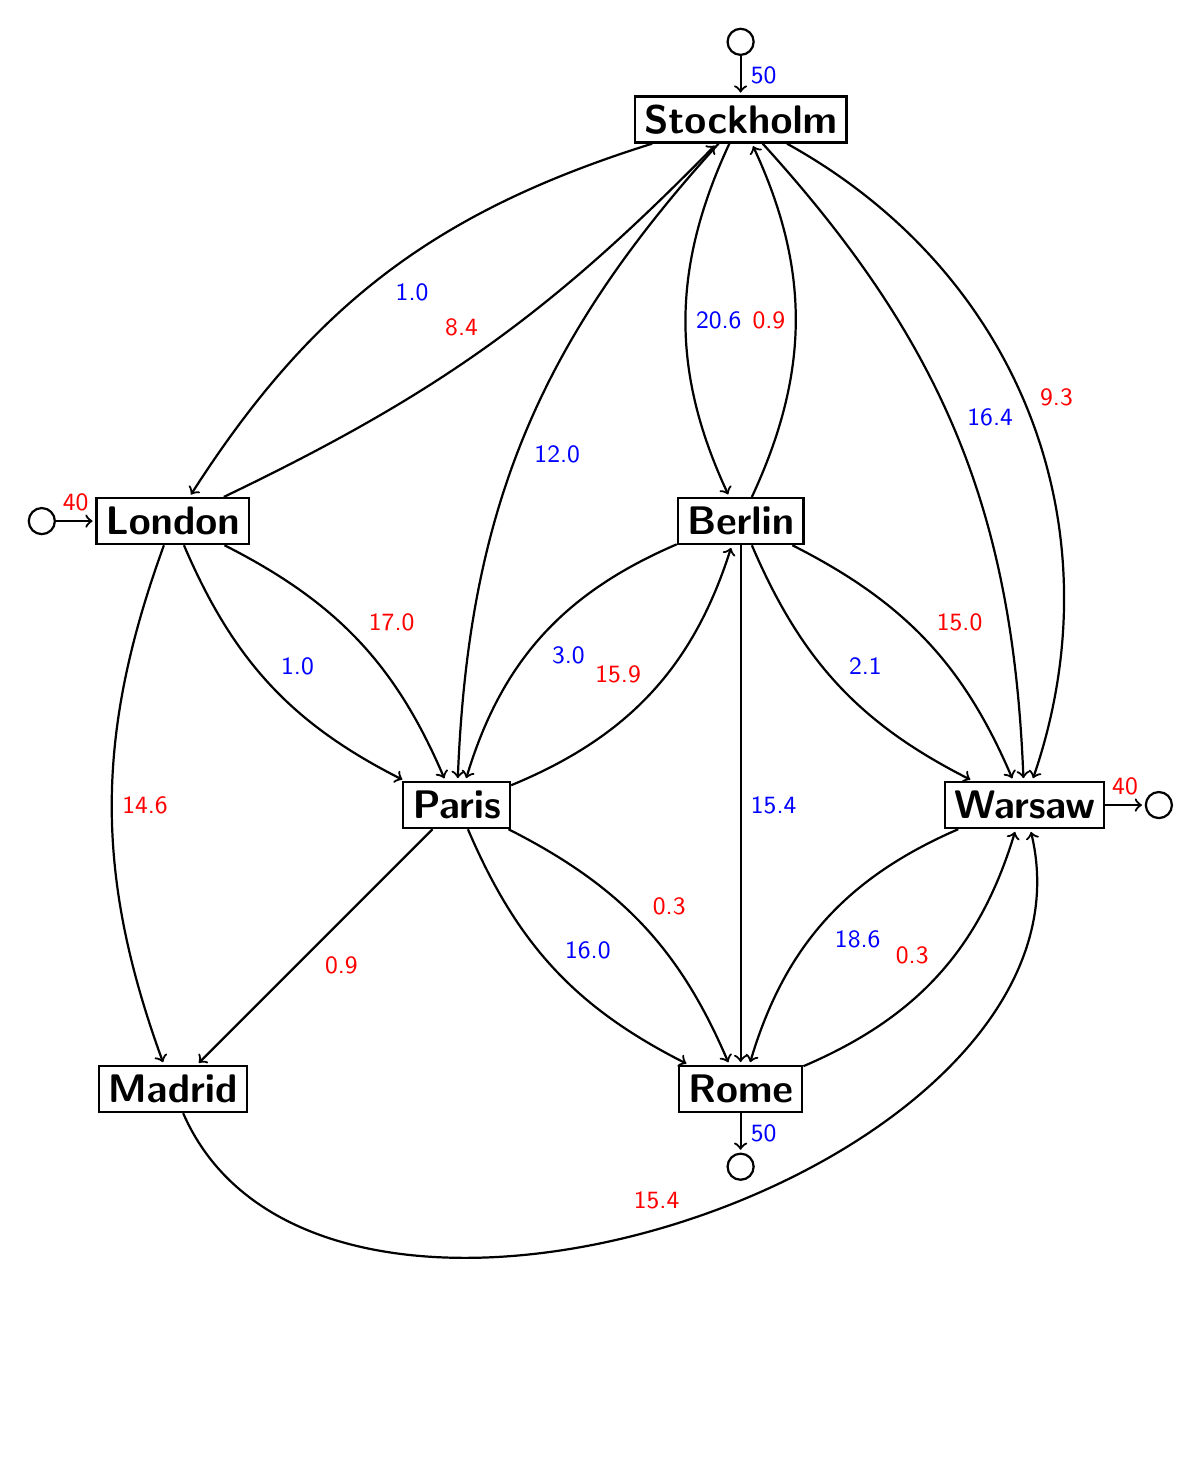
\begin{tikzpicture}[->,thick,shorten >=1pt,auto,node distance=5.1cm,
main node/.style={rectangle,draw,font=\sffamily\Large\bfseries},
plain node/.style={circle,draw,font=\sffamily\Large\bfseries}]
  \node[main node] (1) {Stockholm};
  \node[main node] (2) [below of=1] {Berlin};
  \node[main node] (3) [below right of=2] {Warsaw};
  \node[main node] (4) [below left of=2] {Paris};
  \node[main node] (5) [above left of=4] {London};
  \node[main node] (6) [below right of=4] {Rome};
  \node[main node] (7) [below left of=4] {Madrid};
  \node[plain node] (8)[above =0.5cm of 1] {};
  \node[plain node] (9)[left =0.5cm of 5] {};
  \node[plain node] (10)[right =0.5cm of 3] {};
  \node[plain node] (11)[below =0.5cm of 6] {};

  \path[every node/.style={font=\sffamily\small}]
    (1) edge [bend right=20] node[blue] {1.0} (5)
    	edge [bend right=20] node[blue] {12.0} (4)
     	edge [bend right=25] node[blue] {20.6} (2)
    	edge [bend left=20] node[blue] {16.4} (3)
    	edge [bend left=40] node[red] {9.3} (3)
    (2) edge [bend right=25] node[red] {0.9} (1)
    	edge [bend right=25] node[blue] {3.0} (4)
        edge [bend right=20] node[blue] {2.1} (3)
    	edge [bend left=20] node[red] {15.0} (3)
    	edge node[blue] {15.4} (6)
    (3) edge [bend right=25] node[blue] {18.6} (6)
    	edge node[red] {40} (10)
    (4) edge [bend right=25] node[red] {15.9} (2)
    	edge [bend right=20] node[blue] {16.0} (6)
    	edge [bend left=20] node[red] {0.3} (6)
    	edge node[red] {0.9} (7)
    (5) edge [bend right=10] node[red] {8.4} (1)
    	edge [bend left=20] node[red] {17.0} (4)
    	edge [bend right=20] node[blue] {1.0} (4)
		edge [bend right=20] node[red] {14.6} (7)
	(6) edge [bend right=25] node[red] {0.3} (3)
		edge node[blue] {50} (11)
    (7) edge [bend right=85] node[red] {15.4} (3)
    (8) edge node[blue] {50} (1)
    (9) edge node[red] {40} (5);
\end{tikzpicture}
\end{center}
Figure 2. Result of routing for each type of traffic rounded to the nearest decimal.

Addition to the solution of the variable $x_{i,j,k}$, we also solved for the variable $maxUtility$. The optimal value of utility when routing traffic is $$maxUtility = 0.857$$

To determine whether there is any slack in the network, let us investigate the utility in each link.

\begin{table}[H]
\centering
\caption{Utility for each link}
\label{}
\begin{tabular}{|c|c|} \hline
        Link & Utility				\\ \hline
Sto -- Lon & 85.7\%   \\
Sto -- Par & 85.7\%        \\
Sto -- Ber & 85.7\%     \\
Sto -- War & 85.7\%		\\
Lon -- Par & 85.7\%    \\
Lon -- Mad & 85.7\%       \\
Par -- Ber & 85.7\%    \\
Par -- Mad & 2.8\%     \\
Par -- Rom & 85.7\%    \\
Ber -- War & 65.9\%       \\
Ber -- Rom & 85.7\%     \\
War -- Rom & 85.7\%    \\
Mad -- War & 85.7\%        \\
Mad -- Rom & 0\%      \\ \hline
\end{tabular}
\end{table}

For almost all of the links, the utility is $85.7\%$, which means the traffic is spread evenly. However, there are three links in which there is slack; arcs $(Par,Mad), (Ber,War) \text{ and } (Mad,Rom)$. The connection between Madrid and Rome is not used at all and could be taken away without changing the routing of traffic.

On the other hand, let us now investigate in which links Nett should buy extra capacity in order to create more slack, i.e. decrease the maximum utility. One might think that Nett should invest in all links where the utility is $85.7\%$. Though, this is not true because there are some links where the strain is more severe. In other words, there are some key links in the network which limit the optimal value of the utility.

Along with the solution to the variables in the network problem, we also got \textit{marginal values} for all the capacities in the network respectively. Consider the third constraint in the optimization problem, which controls that the traffic does not exceed the capacity. If we were to move all the variables to the left hand side and keep the constants on the right hand side, the marginal values denote the amount that the objective function change if the right hand side were increased by 1.0. However, the marginal value is only correct for differential changes in the right hand side. In our case, we simply look at which capacities to increase in order to generate the highest decrease in utility.

There are 5 links, with the same marginal value, which we recommend Nett to invest in extra capacity. The links are
$$
(Sto,Lon), (Sto,Par), (Ber,Par), (War,Mad) \text{ and }(War,Rom)
$$

Furthermore, we also discovered the same marginal values for links that do not exist today. If we were to create them, they would have the same influence as the links stated above. For example, Nett should consider buying capacity links between $(Sto,Mad)$ or $(Sto,Rom)$.
\subsection{Results model 2}
\subsection{Result for additional flow}

The maximum available capacity between Berlin and Madrid was found by maximizing the objective function under the constraints in the mathemathical model section 3.2. The resulting optimal solution was calculated using GAMS to be $q = 15$ Gbit/s. Table \ref{table:res2} below presents the resulting system of traffic flow between each node separated into each type of traffic. 

\begin{table}[H]
\centering
\caption{The traffic flow for each type of traffic ($k = 1,2,3$) for each node}
\label{table:res2}
\begin{tabular}{l|lll}
        & $k = 1$   & $k = 2$  & $k = 3$      \\ \hline
Sto -- Par & 14.0   &      &        \\
Sto -- Ber & 14.0   & 3.0  &        \\
Sto -- War & 22.0   & 8.0  &        \\
Lon -- Sto &        & 11.0 &        \\
Lon -- Par &        & 12.0 &        \\
Lon -- Mad &        & 17.0 &        \\
Par -- Ber &        & 11.0 & 11.0   \\
Par -- Mad &        & 1.0  &        \\
Par -- Rom & 14.0   &      &        \\
Ber -- War &        & 14.0 &        \\
Ber -- Rom & 14.0   &      &        \\
War -- Rom & 22.0   &      &        \\
Mad -- Par &        &      & 11.0   \\
Mad -- War &        & 18.0 &        \\
Mad -- Rom &        &      & 4.0    \\
Rom -- Ber &        &      & 4.0 
\end{tabular}
\end{table}

The result is a lot different from the results with only two flows. This is because we are no longer minimizing the utility, but maximizing the additional flow. That means that most of used links are at maximum capacity. The flow is no longer spread evenly.
\subsection{Results model 3}
\subsection{Results for stochastic model}
This section presents the results for the third model (stochastic programming). It sometimes refers to the mathematical model available in the modelisation section.

The first thing to do is to define the different scenarios. Our group chose three different scenarios, called low, medium and high. The low scenario is when all the actual capacities are below the mean by a certain factor $p$. The medium scenario is when the real values are actually the one given. And the high scenario is when the values are above the mean by a factor $p$. So if we reuse the notation defined above :

$$c_{i,j,s} = \left\lbrace \begin{array}{c}
(1-p)c_{i,j} \quad\quad \text{if $s=1$}\\ 
c_{i,j} \quad\quad\qquad\:\:\:\: \text{if $s=2$}\\ 
(1+p)c_{i,j} \quad\quad \text{if $s=3$}
\end{array}\right.$$ 

We also need to assign probability to each scenario. To preserve the fact that the mean value should be $c_{i,j}$, we have that $p_1=p_3$. We chose :
$$p_{s} = \left\lbrace \begin{array}{c}
0.25 \quad\quad \text{if $s=1$}\\ 
0.5 \qquad\:\: \text{if $s=2$}\\ 
0.25 \quad\quad \text{if $s=3$}
\end{array}\right.$$ 

With those scenarios and a chosen factor of $p=0.1$, we get the following expected utility : 
$$\sum_{s=1}^3 p_s\: maxUtility_s = 0.8615$$

The result is a little bit over the utility obtained when we have certainty over the capacities. It is to be expected. Having complete information will yield better results. We also present below the utilities for each scenario :
$$ 
\begin{tabular}{|c|c|c|c|}
\hline 
 & $s=1$ & $s=2$ & $s=3$ \\ 
\hline 
$maxUtility_s$ & 0.952 & 0.857 & 0.779 \\ 
\hline 
\end{tabular} $$

We can see that, the better the scenario, the better the utility. That is quite intuitive. We can also note that if $s=2$ (the capacities are the same as in the deterministic model), then it is possible to route the traffic to find the optimal value found with the deterministic model.

Let us finally look at the proposed traffic. The 40 Gbit/s-flow is given in the table below. In our model, this corresponds to the variables $x_{i,j}$.
\begin{center}
\begin{tabular}{|c|c|c|c|c|c|}
\hline 
i\textbackslash j & Sto & Par & Ber & War & Mad \\ 
\hline 
Sto &  &  &  & 8.762 &  \\ 
\hline 
Lon & 8.762 & 17.333 &  &  & 13.905 \\ 
\hline 
Par &  &  & 17.333 &  &  \\ 
\hline 
Ber &  &  &  & 17.333 &  \\ 
\hline 
Mad &  &  &  & 13.905 &  \\ 
\hline 
\end{tabular} 
\end{center}

Note that this traffic is fixed and cannot depend on the scenarios. We can also check that we have indeed 40Gbit/s leaving Warsaw and 40 Gbit/s entering London. The conservation of flow is also respected. 

Let us compare this solution to the one obtained for the deterministic model. We can see that it does not change much. 

Let us also look at the 50Gbit/s-flow. In our model, this is the variable $y$. It can depend on the scenarios so we will have a different flow for each scenario. The table below gives the results.

\begin{center}
\begin{tabular}{|c|c|c|c|}
\hline 
 & s = 1 & s = 2 & s = 3 \\ 
\hline 
Sto - Lon & 0.667 & 0.667 & 0.667 \\ 
\hline 
Sto - Par & 12 & 12 & 12 \\ 
\hline 
Sto - Ber & 21.429 & 20.381 & 20.381 \\ 
\hline 
Sto - War & 15.905 & 16.952 & 16.952 \\ 
\hline 
Lon - Par & 0.667 & 0.667 &  \\ 
\hline 
Lon - Mad &  &  & 0.667 \\ 
\hline 
Par - Mad &  & 11.333 &  \\ 
\hline 
Par - Rom & 14.190 & 2.857 & 13.524 \\ 
\hline 
Ber - Par & 1.524 & 1.524 & 1.524 \\ 
\hline 
Ber - War & 4.476 & 3.429 & 3.429 \\ 
\hline 
Ber - Rom & 15.429 & 15.429 & 15.429 \\ 
\hline 
War - Mad & 1.524 & 1.524 & 1.524 \\ 
\hline 
War - Rom & 18.857 & 18.857 & 18.857 \\ 
\hline 
Mad - Rom & 1.524 & 12.857 & 2.190 \\ 
\hline 
\end{tabular} 
\end{center}

Once again, we can verify the conservation of flow along with the 50Gbit/s entry in Stockholm and 50Gbit/s output in Rome. We can also see that the solution does not change much if we compare to the one from the basic exercise. 

In conclusion, the solution is not very different from the one obtained in deterministic programming. This is because the scenarios chosen are close to the mean. Also, the same factor is applied to every link in the graph. We could for example consider a scenario where part of the links increase their capacity while other decrease it. We would then have a very different solution. We can also note that, in order to have a feasible region, the factor $p$ must not be too large. For example, if $p=0.2$ then the problem is not feasible. It can easily be seen with the capacities around London. The total mean capacity around London is $11+21+17 = 49$. So if we take 20\% out of that, we get $0.8(11+21+17) = 39.2$. Which is not enough to route a 40 Gbit/s-flow out of London.

\section{Conclusion}
In this report, our group has presented three models to help Nett in finding the best way to route two (or three) flow through a given graph.

In the first model, we are trying to determine the slackness in the graph. We found that the capacities were used up to 85.7\%. This means that it is possible to increase the flow without breaking the capacity constraints.

In the second, we looked for the largest additional traffic the graph could contain. If we choose Madrid and Berlin as end points, we found that the maximal traffic would be of 15 Gbit/s. The traffic between Stockholm and Rome and between London and Warsaw must be rerouted and cannot stay the same as in the first model if we want the optimal solution.

In the last one, we took into account that the capacities given could change and were stochastic parameters. We defined different scenarios and minimized the expected utility. It was of 86.15\%. It is easy to refine the solution by adding more scenarios.


\end{document}